\documentclass[border=3pt,tikz]{standalone}
% Shared look for every TikZ figure in these notes.
% Included by each standalone figure file; also keeps the figures consistent
% with the colours used in the PDF and on the website.

\usepackage{tikz}
\usepackage{pgfplots}
\pgfplotsset{compat=1.18}
\usetikzlibrary{arrows.meta, decorations.markings, decorations.pathmorphing,
                patterns, calc, positioning}
\usepackage{amsmath}

% Series colours are the three validated categorical slots also used by the
% interactive widgets, so a path drawn in the printed notes and the same path on
% the website are the same colour. They clear the colour-vision-deficiency and
% contrast checks as a set; every path is direct-labelled as well, so colour is
% never the only thing carrying identity.
\definecolor{duPurple}{HTML}{68246D}
\definecolor{duBlue}{HTML}{2A78D6}
\definecolor{duRed}{HTML}{EB6834}
\definecolor{duGreen}{HTML}{1BAF7A}
\definecolor{duGrey}{HTML}{4D4D4D}

\tikzset{
  % heavier default lines and arrow tips, so diagrams stay clear when zoomed
  every picture/.append style = {line width=0.7pt, >={Stealth[length=3mm]}},
  axisline/.style   = {-{Stealth[length=3.4mm]}, line width=1.0pt, black},
  path1/.style      = {duBlue,   line width=1.6pt},
  path2/.style      = {duRed,    line width=1.6pt},
  path3/.style      = {duGreen,  line width=1.6pt},
  statedot/.style   = {circle, fill=black, inner sep=1.8pt},
  arrowhead/.style  = {decoration={markings,
                        mark=at position #1 with {\arrow{Stealth[length=3.4mm]}}},
                       postaction={decorate}},
  lbl/.style        = {font=\normalsize},
  slbl/.style       = {font=\small, duGrey},
  workfill/.style   = {duPurple, opacity=0.16},
}

% larger labels in plots as well
\pgfplotsset{every axis/.append style={label style={font=\normalsize}, tick label style={font=\small}, line width=0.9pt}}

% P6.5 solution sketch: the argon in the bulb is the system; it loses heat q
% to the 20 C room while it cools from 80 C to 20 C.
\begin{document}
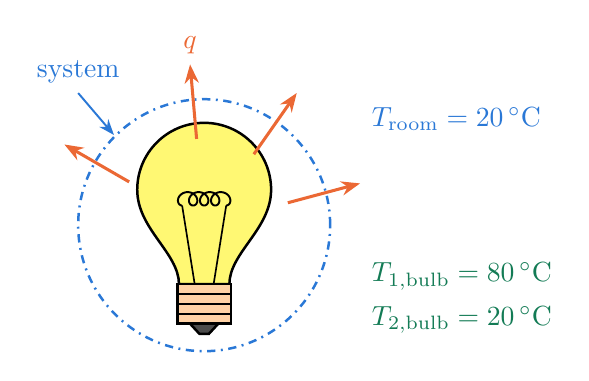
\begin{tikzpicture}[x=1cm,y=1cm,
    q/.style={-{Stealth[length=2.4mm]}, line width=1.1pt, duRed}]
  % --- bulb ---------------------------------------------------------------
  \draw[line width=0.9pt, fill=yellow!55]
    (-0.32,-0.75) .. controls (-0.32,-0.35) and (-0.85,-0.05) .. (-0.85,0.45)
    arc[start angle=180, end angle=0, radius=0.85]
    .. controls (0.85,-0.05) and (0.32,-0.35) .. (0.32,-0.75) -- cycle;
  % filament and its supports
  \draw[line width=0.6pt] (-0.12,-0.75) -- (-0.28,0.25) (0.12,-0.75) -- (0.28,0.25);
  \draw[line width=0.7pt, smooth, domain=0:1440, samples=240, variable=\t]
    plot ({-0.28 + 0.56*\t/1440 - 0.085*sin(\t)}, {0.25 + 0.085*(1 - cos(\t))});
  % screw base
  \draw[line width=0.9pt, fill=orange!35] (-0.34,-0.75) rectangle (0.34,-1.25);
  \foreach \y in {-0.875,-1.0,-1.125} \draw[line width=0.6pt] (-0.34,\y) -- (0.34,\y);
  \draw[line width=0.9pt, fill=black!70] (-0.18,-1.25) -- (0.18,-1.25) -- (0.06,-1.38) -- (-0.06,-1.38) -- cycle;
  % --- system boundary ------------------------------------------------------
  \draw[duBlue, dash dot, line width=0.9pt] (0,0) circle (1.6);
  \node[lbl, duBlue] (sys) at (-1.6,1.95) {system};
  \draw[-{Stealth[length=2mm]}, line width=0.7pt, duBlue] (sys.south) -- (135:1.62);
  % --- heat lost to the room ---------------------------------------------
  \foreach \a in {150, 95, 55, 15} \draw[q] (\a:1.1) -- (\a:2.05);
  \node[lbl, duRed, above] at (95:2.05) {$q$};
  % --- temperatures ------------------------------------------------------
  \node[lbl, duBlue, anchor=west] at (2.0,1.35) {$T_\text{room} = 20\,^\circ$C};
  \node[lbl, duGreen!70!black, anchor=west] at (2.0,-0.65) {$T_{1,\text{bulb}} = 80\,^\circ$C};
  \node[lbl, duGreen!70!black, anchor=west] at (2.0,-1.2) {$T_{2,\text{bulb}} = 20\,^\circ$C};
\end{tikzpicture}
\end{document}
